\chapter{Technology Overview} \label{chap:tech} %% chapter 3
\hspace {5mm}

%% ADD LINK TO sections
After a brief introduction, encompassing the history, and some of the requirements in the technologies that support the developed work, this chapter focuses on giving a detailed description of the infrastructure supporting 
the developed work. This chapter is organized in the following matter: in the first section, we focus on SDN/NFV platforms, and the OpenFlow platform; in the second section, an introduction to cloud computing is the main topic,
while also clarifying some of concepts of containerization and virtualization, and how these techniques support the SDN model; in section three, some methods of describing links are explained; in section four, there is an 
analysis of how to monitor and control the SDN platform; and finally in section five we describe how some databases can serve as a backend, and also presenting some interesting new alternatives to the most common ones.

\section {SDN/ NFV}


\begin{figure}[!tbph]
  \centering
  {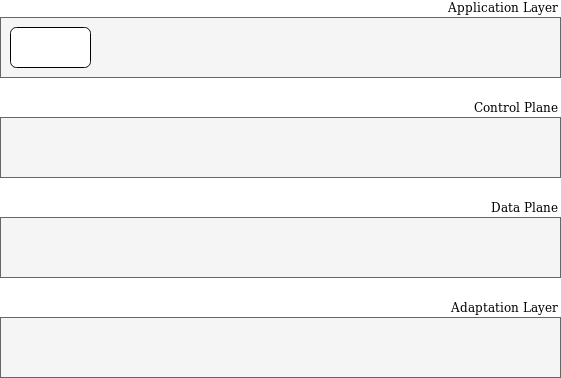
\includegraphics[width=0.4\textwidth]{technology/sdnlayers}\label{fig:net_trad}}
\end{figure}

\subsection {OpenFlow}
\section {Cloud computing and SaaS}
\subsection {Containerization vs Virtualization}
\section {Link discovery and control}
\section {Infrastructure Management/ Configuration}
\subsection {Data Models}
\subsection {Management Protocols}
\subsubsection {SNMP}
\subsubsection {NETCONF}
\subsubsection {gRPC}
\section {Databases and SDN} %% ??

%% PRESENT PROMETHEUS
